\documentclass[conference]{IEEEtran}
\IEEEoverridecommandlockouts
% The preceding line is only needed to identify funding in the first footnote. If that is unneeded, please comment it out.
\usepackage{cite}
\usepackage{amsmath,amssymb,amsfonts}
\usepackage{algorithmic}
\usepackage{graphicx}
\usepackage{textcomp}
\usepackage{xcolor}
\usepackage{tgtermes}
\usepackage{mathptmx}
\usepackage{mathpazo}
\usepackage{fontspec}
%\renewcommand{\baselinestretch}{0.92}
\makeatletter
\newcommand{\linebreakand}{%
  \end{@IEEEauthorhalign}
  \raggedright \mbox{}\par
  \mbox{}\raggedright\begin{@IEEEauthorhalign}
}
\makeatother

\def\BibTeX{{\rm B\kern-.05em{\sc i\kern-.025em b}\kern-.08em
    T\kern-.1667em\lower.7ex\hbox{E}\kern-.125emX}}
\begin{document}

\title{Automatic Language Identification on Audio Signals}
%\IEEEoverridecommandlockouts
%\IEEEpubid{\makebox[\columnwidth]{978-1-7281- -/20/\$31.00~\copyright{}2020 IEEE \hfill} \hspace%{\columnsep}\makebox[\columnwidth]{ }}



\author{
\linebreakand
\IEEEauthorblockN{Khaing Zar Mon}
\IEEEauthorblockA{
\textit{ME-IST-5}\\
\textit{Department of Information Science} \\
\textit{University of Technology (Yatanarpon Cyber City)}\\
khaingzarmon@utycc.edu.mm}
\and
\IEEEauthorblockN{May Phyu Khin}
\IEEEauthorblockA{
\textit{ME-IST-7}\\
\textit{Department of Information Science} \\
\textit{University of Technology (Yatanarpon Cyber City)}\\
mayphyukhin@utycc.edu.mm}
\and
\IEEEauthorblockN{Myo Mar Thinn}
\IEEEauthorblockA{
\textit{ME-IST-3}\\
\textit{Department of Information Science} \\
\textit{University of Technology (Yatanarpon Cyber City)}\\
myomarthinn@utycc.edu.mm}
\and
\IEEEauthorblockN{Ei Thandar Phyu}
\IEEEauthorblockA{
\textit{ME-IST-2}\\
\textit{Department of Information Science} \\
\textit{University of Technology (Yatanarpon Cyber City)}\\
eithandarphyu@utycc.edu.mm}
\and
\IEEEauthorblockN{Nang Aeindray Kyaw}
\IEEEauthorblockA{
\textit{ME-IST-6}\\
\textit{Department of Information Science} \\
\textit{University of Technology (Yatanarpon Cyber City)}\\
nangaeindraykyaw@utycc.edu.mm}
}
\maketitle
\begin{abstract}
The purpose of our study is to identify which language is spoken from a speech sample, based solely on the acoustic information conveyed by the speech signal. There are many characteristics of speech that could be used to identify languages. Languages are made up of different sounds that form phonemes, so it is possible to distinguish languages based on the acoustic features present in the speech signal. We decided to study language identification of four different languages, namely English, Chinese, Myanmar (Burmese) and Shan (Tai Long). In this study, three different approaches were used to carry out the experiments. The first one is language identification from Mel Frequency Cepstral Coefficients (MFCC) using Keras Library. In the second approach, we use waveforms of raw audio signals as input to a Residual Neural Networks (ResNets). For the last approach, we use spectrograms of our audio data as input to ResNets which in turn is trained for language identification. According to our experimental results, all the approaches give promising results. The first approach, language identification with MECC using Keras, and the last approach, identification using spectrograms, give 100\% testing accuracy. We expect a more useful system can be developed as more data (with more language classes) comes available in the future.
\end{abstract}

\begin{IEEEkeywords}
Language Identification, Residual Neural Networks (ResNets), Mel Frequency Cepstral Coefficients (MFCC) 
\end{IEEEkeywords}

\section{Introduction}
Recently, voice assistants have become a staple in the flagship products of many big technology companies such as Google, Apple, Amazon, and Microsoft. One challenge for intelligent assistants, like Siri or the Google Assistant, is that the language that a speaker is using needs to be preset. To improve user experience on this and similar tasks such as automated speech detection or speech to text transcription, automatic language detection is a necessary first step. Moreover, emergency call routing can be one of the applications of language identification, where the response time of a fluent native operator might be critical. The main motivation is to study language identification from audio data using different Deep Learning approaches.

Finding a dataset of audio clips in various languages sufficiently large for training a network was an initial challenge for this task. Due to the difficulty to get open-source audio corpus for various languages, we only use audio corpus with four different languages, namely English, Chinese, Myanmar (Burmese) and Shan (Tai Long).
In this project, we studied the implementation and evaluation of three different language identification models and compared the results. Firstly, we extracted Mel Frequency Cepstral Coefficients (MFCC) features from our audio data and trained with Keras Library to build a language identification model. We also studied to use Residual Neural Networks (ResNets) for language identification and built two models with ResNets. Waveforms of audio data are used as input of the second model and spectrograms of audio data are used as input of the third model. 

The structure of this paper is organized as follows. Related works of language identification for different languages using audio data are presented in the upcoming section. Section~\ref{Sec:Methodology} describes the methodologies used in the language identification experiments. Later, in Section~\ref{Sec:Experiments}, we present corpus preparation and data pre-processing together with feature extraction techniques used for the experiments. The experimental results along with some discussions are described in Section~\ref{Sec:ResultDiscussion}. Eventually, in Section~\ref{Sec:Conclusion}, we conclude our works showing promising results.

\section{Related Work}\label{Sec:RelatedWork}
Audio language identification systems are usually based on identity vector systems \cite{b4} and \cite{b9}. Spectorgram-based language classification are also performed on neural network models\cite{b1,b2} and \cite{b11}. Using deep neural network, language identification based on audio signals were also presented in \cite{b5,b8} and \cite{b10}. In \cite{b12}, identification results using Long Short-Term Memory (LSTM) Recurrent Neural Network provided better performance than on identity vector systems. Based on related studies, these neural networks based systems are more convenient to language identification tasks because they achieved highest accuracy rates. Therefore, we performed language identification based on audio files and images (spectrograms and waveforms) for different four languages.

\section{Methodology}\label{Sec:Methodology} 

In this section, we describe the methodologies used in language classification on audio features.

\subsection{Audio Feature Extraction}\label{SubSec:AudioFeature}
Before an audio signal can be classified, the features within that signal first need to be extracted and analysed. These features represent the characteristics of the audio signal and will ultimately decide the class of that signal. The techniques employed during feature extraction can either involve the analysis of the actual waveform of the audio signal, or the analysis of the spectral representation of the audio signal. During the feature extraction stage there is reduction of data from the audio signal as sound data contains much redundancy \cite{b3}. This is done by breaking down the audio signal into successive short-time or short-term windows or frames, which are generally no larger than 100ms \cite{b6}. A set of features are then calculated for each frame, resulting in a feature vector \cite{b12}.

\subsection{Mel-frequency Cepstral Coefficients (MFCC)}\label{SubSec:MFCC}
MFCC is one of the most important method to extract a feature of an audio signal and is used majorly whenever working on audio signals. In practise, MFCCs are the discrete cosine transform coefficients of the mel-scaled log-power spectrum. MFCC is a technique based on human hearing behavior that cannot recognize frequencies  over 1 kHz. MFCC are based on the difference of frequencies that the human ear can distinguish. The signal is expressed in the MEL scale, this scale is based on the perception of the pitches in an equally spaced intervals judged by observers \cite{b7}. MFCCs have been widely used in speech recognition, speaker clustering and many other audio analysis applications.

\subsection{Transfer Learning}\label{SubSec:TransferLearning}
Transfer learning is a method to leverage the generic knowledge acquired by a model trained on massive datasets to develop a more task-specific knowledge using only a limited amount of new data. While generic knowledge is used to detect low-level features in an image, such as edges and curves, task-specific knowledge enables the model to recognize higher-level features, such as the shape of a hand, type of spectrogram and wave images. Generic knowledge is formed in the lower layers of the CNN (near the input image), while specific knowledge grows in the upper layers, near the classifier (the output)\cite{b14}.
	 
\subsection{ResNet-50}\label{SubSec:ResNet}
ResNet-50 is the Residual Network with 50 layers. Convolutional neural networks (CNN), a type of deep learning network with excellent performance in detecting features in images\cite{b15}. There are many pre-trained models like VGG, Inspection-V3, MobileNet,ResNet and so on. These pre-trained models saving us the time and expense of having to do the training from scratch. ResNet-50 is ideal for speed, accuracy and can load a pretrained version of the network trained on more than a million images from the ImageNet database. The pretrained network can classify images into 1,000 object categories, such as keyboard, mouse, pencil, and many animals. As a result, the network has learned rich feature representations for a wide range of images. The network has an image input size of 224-by-224\cite{b16}.

\section{Experiments}\label{Sec:Experiments}
In this section, the experiment settings for the audio language identification are described. The experiment consisted of four main parts: preparation of audio data, audio featuring, classification of different languages based on audio files and classification of different languages based on images (spectrograms and waveforms).

\subsection{Audio Data Preparation}\label{SubSec:AudioCorpus}
For our experiments, audio clips were gathered in Burmese, English, Shan, and Chinese. We used μtopia - Microblog Translated Posts Parallel Corpus (Release V1.1 - 19/09/2013) for English and Chinese audio files. For Shan language, we prepared audio files by recording three native Shan speakers. Myanmar audio files were collected from weather broadcasts. Speakers had various accents and were of different genders. For each language, there were 1,000 audio files. All audio files were sampled at a rate of 16kHz with a mono channel. The audio files were saved as WAV files.   

\subsection{Audio Featuring}\label{SubSec:AudioFeaturing}
In this experiment, the audio features of audio signal are extracted from the audio files for audio based language classification. We used Librosa which is a python package used for analyzing and extracting features of an audio signal. For image based classification, the audio files were represented in the forms of images (spectrograms and waveforms). A spectrogram is a detailed view of audio which displays changes in the frequencies in a signal over time. A waveform is an image that represents an audio signal showing the changes in amplitude over a certain amount of time. The spectrograms of the audio files were extracted using the Sound eXchange (SoX, Swiss Army knife of sound processing programs) command line utility \cite{b10}. Using the FFmpeg cross-platform solution, the audio files were converted to the waveforms. Some spectrograms of Shan and Chinese audio files are described in Fig.~\ref{fig:ShanSpec} and Fig.~\ref{fig:ChinaSpec} respectively. In Fig.~\ref{fig:BurmaWav} and Fig.~\ref{fig:EngWav}, waveforms of Burmese and English languages are shown.

\begin{figure}[t]
\centerline{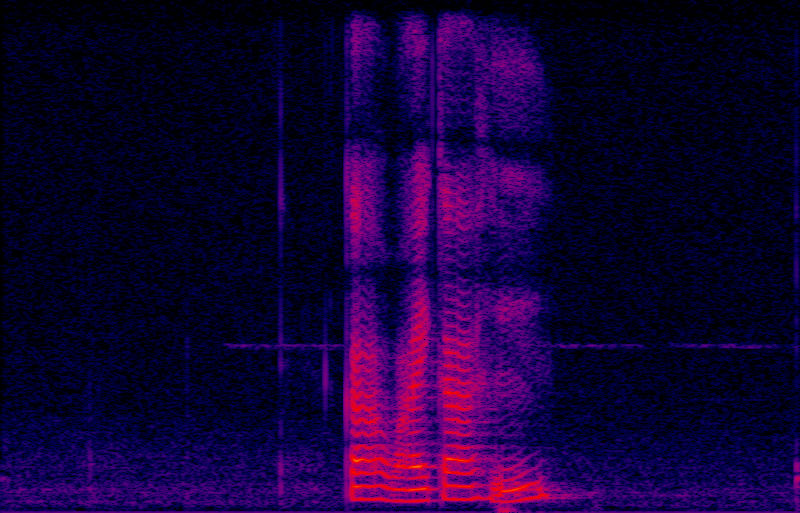
\includegraphics[width=90mm,height=3cm]{shanspec.jpg}}
\caption{Spectrogram of Shan Audio File}
\label{fig:ShanSpec}
\end{figure}

\begin{figure}[t]
\centerline{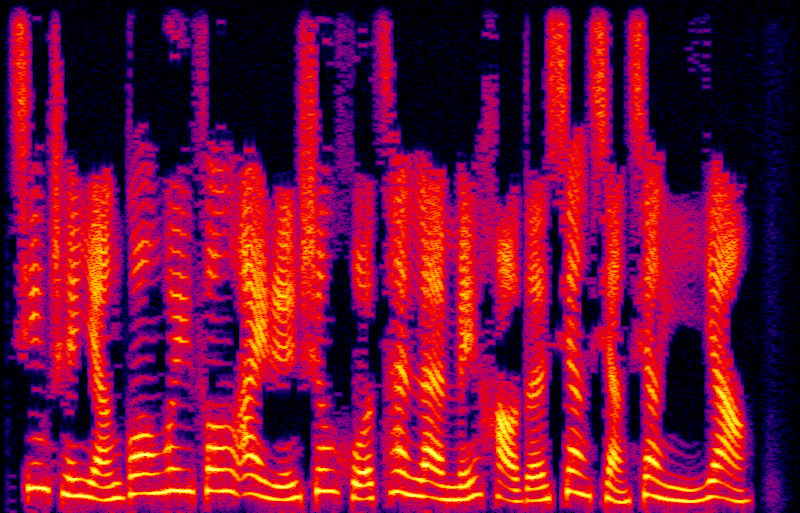
\includegraphics[width=90mm,height=3cm]{chinaspec.jpg}}
\caption{Spectrogram of Chinese Audio File}
\label{fig:ChinaSpec}
\end{figure}

\begin{figure}[t]
\centerline{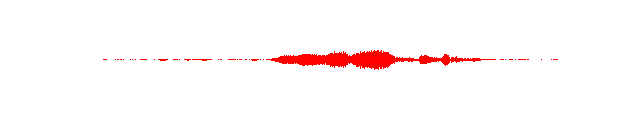
\includegraphics[width=90mm,height=3cm]{burmawav.png}}
\caption{Waveform of Burmese Audio File}
\label{fig:BurmaWav}
\end{figure}

\begin{figure}[t]
\centerline{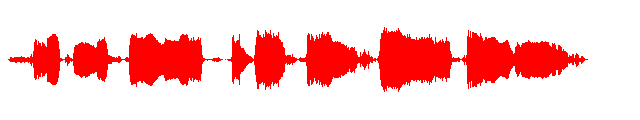
\includegraphics[width=90mm,height=3cm]{engwav.png}}
\caption{Waveform of English Audio File}
\label{fig:EngWav}
\end{figure}

\subsection{Classification of different languges based on audio files}\label{SubSec:AudioClassification}
In our experiments, the total audio files used for four languages are 4,000. The integrated development environment (IDE) used for the process is Google Colaboratory or Google Colab in short. Google Colab is a free Jupyter notebook environment that requires no setup and runs entirely in the cloud. With Google Colab, it is possible to write and execute code, save and share the analyses, and access powerful computing resources, all for free from the browser.

The audio features are extracted from the audio files. We used Librosa for analyzing and extracting features of an audio signal. Librosa is a python package used for audio analysis. After extracting features, the data is standardized by removing the mean and scaling to unit variance. Standardization is useful for negative-value results.

The language is predicted based on the Convolutional Neural Network (CNN). There are 4 layers in this network. The first one is an input layer therefore, input size is equal to the numbers of features used. Then there are 2 hidden layers and the last layer is an output layer. The output layer has 4 neurons as we are classifying into 4 languages. We applied rectified linear unit (ReLU) for activation and for the classification we are using softmax. The optimizer is the adam and the loss function is the sparse categorical cross entropy. We passed the data to the model with epochs 20 and batch size 128. The model gives us percentage by how much that  utterance matches to each language. The highest percentage for the given utterance is the final result. Finally, we got the accuracy by the model that can correctly predict the language of given utterance based on the features extracted. We used tensorflow package at the backend. 

\subsection{Classification of different languges based on spectrogram and waveform images}
We used GPU and tensorflow framework for image classification. Input image size for ResNet-50 is 224 $\times$ 224 and batch size 16 is deployed to process in one iteration. We used 3600 images for training samples, 400 images for validation (close testing) and 400 images for testing samples (open testing) belonging to four classes (Burmese, Chinese, English and Shan). In our experiments, ImageDataGenerator was applied for training pictures with data augmentation, to get more training data by applying different transformations to the existing pictures (rotation, shift, zoom, etc.). Since we had four classes, we chose 'categorical\_crossentropy' as the loss function and epochs 50. 
	
We recreate the top layer (classifier) with one additional neuron for the new category and retrain the upper layers with pictures (spectrograms and wave forms). In order to avoid class imbalance, we train the similar number of images.

\section{Results and Discussion}\label{Sec:ResultDiscussion}
Experimental results of proposed system are explained in this section. In our experiments, language identification using MFCC features was performed on 3200 training data and 800 testing data for Burmese, Shan, English and Chinese languages. We also performed classification on spectrogram images and waveform images with 3200 traing data, 400 validation data and 400 testing data. Accuracy was calculated for each classification method as in equation \ref{eq:acc_eq}.
\begin{equation}
Accuracy = \frac{Number\: of\: correct predictions}{Total\: Number\: of\: predictions}\label{eq:acc_eq}
\end{equation}

A comparison of the classification accuracies is shown in Table \ref{table:acc_tb}. Bold numbers indicate the highest scores among the three approaches. 
\begin{table}[htbp]
\caption{Comparison of identification accuracies}
\begin{center}
\begin{tabular}{|c|c|}
\hline
\bf{Method}&\bf{Accuracy (\%) } \\
\hline
Identification on MFCC features&\textbf{100\% } \\
\hline
Identification on wave images&96.5\%  \\
\hline
Identification on spectrogram images&\textbf{100\% }\\
\hline
\end{tabular}
\label{table:acc_tb}
\end{center}
\end{table}

For four languages, the precision, recall and F1 score were presented in order to determine the performance. Precision is the ratio of correctly predicted positive observations to the total predicted positive observations. Recall is the ratio of correctly predicted positive observations to the all observations in actual class. F1 score is the weighted average of precision and recall. The calculations of precision, recall and F1 score are as in equation \ref{eq:pre_eq}, \ref{eq:rec_eq} and \ref{eq:f_eq}.
\begin{equation}
Precision = \frac{True\: Positive}{True\: Positive\: +\: False\: Postive}\label{eq:pre_eq}
\end{equation}
\begin{equation}
Recall = \frac{True\: Positive}{True\: Positive\: +\: False\: Negative}\label{eq:rec_eq}
\end{equation}
\begin{equation}
F1 score = \frac{2*(Recall*Precision)}{Recall+ Precision}\label{eq:f_eq}
\end{equation}
\begin{table}[htbp]
\caption{Precision, Recall and F1 score}
\begin{center}
\begin{tabular}{|c|c|c|c|}
\hline
\textbf{Features}&\textbf{Precision} &\textbf{Recall} &\textbf{F1 score} \\
\hline
MFCC &\textbf{1} &\textbf{1} &\textbf{1} \\
\hline
waveform images &0.97 &0.96 &0.96\ \\
\hline
spectrogram images &\textbf{1} &\textbf{1} &\textbf{1}  \\
\hline
\end{tabular}
\label{table:prf_tb}
\end{center}
\end{table}

As in Table \ref{table:acc_tb} and \ref{table:prf_tb}, it can be assumed that the scores of the three approaches are comparable. Identification with MFCC feature and identification using spectrogram achieved the highest accuracy. For Burmese, English, Shan and Chinese languages, these two approaches could correctly classify all audio files of speakers with various accents. For image based identification, classification on the spectrogram images outperfomed over that of waveforms. The language identificaiton on the waveform images could also correctly identify Burmese and Shan voices. However, it contained errors in classification of English and Chinese languages.

\section{Conclusion}\label{Sec:Conclusion}
This work shows the study of three different languge identification models along with their performances in classifying four languages, English, Chinese, Myanmar (Burmese) and Shan (Tai Long). Robust performance can be accomplished with minimal pre-processing. We believe that these models can be extended to classify more languages so long as sufficient, representative training and validation data is available.

\begin{thebibliography}{00}
\bibitem{b1}Alexandra Draghici,and Hanna Lukashevich, "A Study on Spoken Language Identification using Deep Neural Networks", 2020-July.
\bibitem{b2}Bartz, C., Herold, T., Yang, H., Meinel, "Language identification using deep convolutional recurrent neural networks" in Neural Information Processing. LNCS, vol. 10639, pp. 880–889. Springer, Cham (2017).
\bibitem{b3}D. Gerhard, Audio signal classification: History and current techniques: Citeseer, 2003.
\bibitem{b4}D. Martinez, O. Plchot, L. Burget, O. Glembek and P. Matejka, "Language recognition in iVectors space", Proc. Interspeech, 2011-Aug.
\bibitem{b5}Fred Richardson, Doug Reynolds and Najim Dehak, "A Unified Deep Neural Network for Speaker and Language Recognition", in INTERSPEECH 2015.
\bibitem{b6}J. J. Burred and A. Lerch, "Hierarchical automatic audio signal classification,"Journal of the Audio Engineering Society, vol. 52, pp. 724-739, 2004.
\bibitem{b7}J. Martinez, H. Perez, E. Escamilla and M. M. Suzuki, "Speaker recognition using Mel frequency Cepstral Coefficients (MFCC) and Vector quantization (VQ) techniques," CONIELECOMP 2012, 22nd International Conference on Electrical Communications and Computers, Cholula, Puebla, 2012, pp. 248-251, doi: 10.1109/CONIELECOMP.2012.6189918.
Spectrogram
\bibitem{b8}Julien Boussard, Andrew Deveau, Justin Pyron, "Methods for Spoken Language Identification",in 2017-Dec.
\bibitem{b9}N. Dehak, P. J. Kenny, R. Dehak, P. Dumouchel and P. Ouellet, "Front-End Factor Analysis for Speaker Verification," in IEEE Transactions on Audio, Speech, and Language Processing, vol. 19, no. 4, pp. 788-798, May 2011.
\bibitem{b10}Rutuja Ubale, Vikram Ramanarayanan, Yao Qian, Keelan Evanini, Chee Wee Leong, and Chong Min Lee, "Native Language Identification from Raw Waveforms using Deep Convolutational Neural Networks with Attentive Pooling", in IEEE 2019.
\bibitem{b11}Shauna Revay and Matthew Teschke, "Multiclass Language Identification using Deep Learning on Spectral Images of Audio Signals", 2019-May. 
\bibitem{b12}T. Giannakopoulos, "PyAudioAnalysis. A Python library for audio feature extraction, classification, segmentation and applications," PloS one, vol. 10, p.e0144610, 2015.
\bibitem{b13}Zazo R, Lozano-Diez A, Gonzalez-Dominguez J, T. Toledano D, Gonzalez-Rodriguez J, "Language Identification in Short Utterances Using Long Short-Term Memory (LSTM) Recurrent Neural Networks", in 2016-Jan.
\bibitem{b14}https://medium.com/analytics-vidhya/how-to-train-your-resnet-the-jindo-dog-50551117381d
\bibitem{b15}https://www.quora.com/What-is-ResNet-50-How-does-it-work-and-how-many-layers-does-it-have
\bibitem{b16}https://www.mathworks.com/help/deeplearning/ref/resnet50.html
\end{thebibliography}
\vspace{12pt}
\end{document}
